\documentclass[10pt,a4paper]{article}
% =================================================================
% DS5006 Team Project --- Report Template
% Sub-Question 1 (SQ1) Evaluation: Numerical Meaning of Ordinal Rating Scales
% =================================================================
\usepackage[margin=2.2cm]{geometry}
\usepackage{amsmath,amssymb}
\usepackage{graphicx}
\usepackage{booktabs,tabularx}
\usepackage{xcolor}
\usepackage{enumitem}
\usepackage[numbers]{natbib}
\usepackage{tikz}
\usetikzlibrary{arrows.meta, positioning, calc}
\usepackage{hyperref}
\hypersetup{colorlinks=true,linkcolor=blue!50!black,citecolor=blue!50!black,urlcolor=blue!50!black}
\setlist{itemsep=0.5pt,topsep=2pt,parsep=0pt}
\linespread{0.94}
\setlength{\parskip}{1pt plus 0.5pt minus 0.5pt}
\renewcommand{\arraystretch}{0.85}

\newcommand{\teamname}{Team Arch}
\newcommand{\projecttitle}{Airline Passenger Satisfaction Prediction}

\title{\textbf{\projecttitle}\\[4pt]\large DS5006 Machine Learning --- Team Project Report}
\author{\teamname\\[2pt]
\small Ishwer Dutt \quad Krishna M \quad Rajavel K\\
\small Department of Data Science, Indian Institute of Technology Palakkad}
\date{\today}

\begin{document}
\maketitle

\begin{abstract}

\end{abstract}

% =================================================================
\section{Introduction and scientific questions}

\begin{description}[leftmargin=1.2em,style=nextline]
\item[Q1.] Does the numerical meaning of an ordinal rating scale matter?
      \textbf{Hypothesis:} Predictions will not be completely invariant to numerical spacing, as the effect may differ across model classes. Tree-based models primarily use ordering and split thresholds,they must be invarient to these transformations, whereas linear and kernel methods
use numerical distances
      \textbf{Falsified if:} Linear models show zero shift ($\Delta\text{ROC-AUC} = 0$, no flips) or trees produce flips under
      monotonic scaling.
\end{description}

% =================================================================
\section{Related work}

% =================================================================
\section{Data}
We evaluate the Kaggle Aviation Passenger Satisfaction benchmark ($N = 699{,}635$ records, 21 predictors, binary target \texttt{satisfaction}: $55.6\%$ dissatisfied, $44.4\%$ satisfied). Preprocessing is strictly encapsulated in an isolated \texttt{Column\-Transformer} across 5 repeated stratified $80/20$ splits (seeds $\{42, 123, 2025, 7, 99\}$; $N_{\text{train}} = 559{,}708$, $N_{\text{test}} = 139{,}927$). Table~\ref{tab:feature_specs} details the feature taxonomy, domains, and column specifications.

\begin{table}[h]
\centering
\footnotesize
\renewcommand{\arraystretch}{0.82}
\setlength{\tabcolsep}{3.5pt}
\caption{\textbf{Feature Specifications and Column Taxonomy ($N=699{,}635$).}}
\label{tab:feature_specs}
\begin{tabularx}{\linewidth}{@{}l l >{\raggedright\arraybackslash}X c >{\raggedright\arraybackslash}X@{}}
\toprule
\textbf{Feature / Column} & \textbf{Type} & \textbf{Domain / Scale} & \textbf{Nulls} & \textbf{Preprocessing / Stream} \\
\midrule
\texttt{satisfaction} (Target) & Binary & 0: Dissatisfied (55.6\%), 1: Satisfied (44.4\%) & 0 & Target label \\
\midrule
12 Service Items\footnotemark & Ordinal & $\{0..5\}$ ($0 = \text{NA}$, $1\text{--}5$ Likert) & 0 & Scaled vs. raw unscaled $g(v)$ \\
\texttt{Baggage handling} & Ordinal & $\{1..5\}$ (Strictly positive) & 0 & Scaled vs. raw unscaled $g(v)$ \\
\midrule
\texttt{Age} & Continuous & Range: $7\text{--}85$ years & 0 & Standardized ($\mu=0,\sigma=1$) / Raw \\
\texttt{Flight Distance} & Continuous & Range: $31\text{--}4983$ miles & 0 & Standardized ($\mu=0,\sigma=1$) / Raw \\
\texttt{Departure Delay} & Continuous & Range: $0\text{--}1592$ minutes & 0 & Standardized ($\mu=0,\sigma=1$) / Raw \\
\texttt{Arrival Delay} & Continuous & Range: $0\text{--}1584$ minutes & 292 & Median imputed + Standardized \\
\midrule
\texttt{Gender} & Categorical & Female (50.7\%), Male (49.3\%) & 0 & One-Hot Encoded (drop='first') \\
\texttt{Customer Type} & Categorical & Loyal (81.7\%), Disloyal (18.3\%) & 0 & One-Hot Encoded (drop='first') \\
\texttt{Type of Travel} & Categorical & Business (69.0\%), Personal (31.0\%) & 0 & One-Hot Encoded (drop='first') \\
\texttt{Class} & Categorical & Business (47.8\%), Eco (45.0\%), Eco Plus (7.2\%) & 0 & One-Hot Encoded \\
\bottomrule
\end{tabularx}
\end{table}
\footnotetext{The 12 standard ordinal items: \emph{Inflight wifi service}, \emph{Departure/Arrival time convenient}, \emph{Ease of Online booking}, \emph{Gate location}, \emph{Food and drink}, \emph{Online boarding}, \emph{Seat comfort}, \emph{Inflight entertainment}, \emph{On-board service}, \emph{Leg room service}, \emph{Checkin service}, and \emph{Cleanliness}.}

% =================================================================
\section{Methodology}
To test the effect of ordinal scale spacing across diverse inductive biases, we examine five distinct model families totaling 100 model fits (5 splits $\times$ 4 encodings $\times$ 5 models):
\begin{enumerate}[leftmargin=1.2em]
    \item \textbf{Majority Class Baseline:} Predicts the empirical training mode ($55.6\%$ dissatisfied), providing a null benchmark ($0.5000$ ROC-AUC, $0.5000$ Balanced Accuracy).
    \item \textbf{Logistic Regression:} Standardized L2-regularized logistic regression ($C=1.0$, L-BFGS solver, tolerance $10^{-4}$). 
    \item \textbf{Linear SVM:} \texttt{LinearSVC} with squared hinge loss ($C=1.0$, max iter 2,000). Probability outputs are calibrated using 2-fold out-of-fold Platt sigmoid scaling.
    \item \textbf{Decision Tree:} CART classifier with max depth 15, minimum samples per leaf 20, and Gini impurity splitting. Features are passed unscaled.
    \item \textbf{Random Forest:} Bagged ensemble of 100 CART trees with max depth 20, minimum samples per leaf 10, and $\sqrt{p}$ random feature subsampling.
\end{enumerate}

Figure~\ref{fig:pipeline} details the end-to-end experimental architecture and paired evaluation pipeline.

\begin{figure}[t]
\centering
\resizebox{\linewidth}{!}{
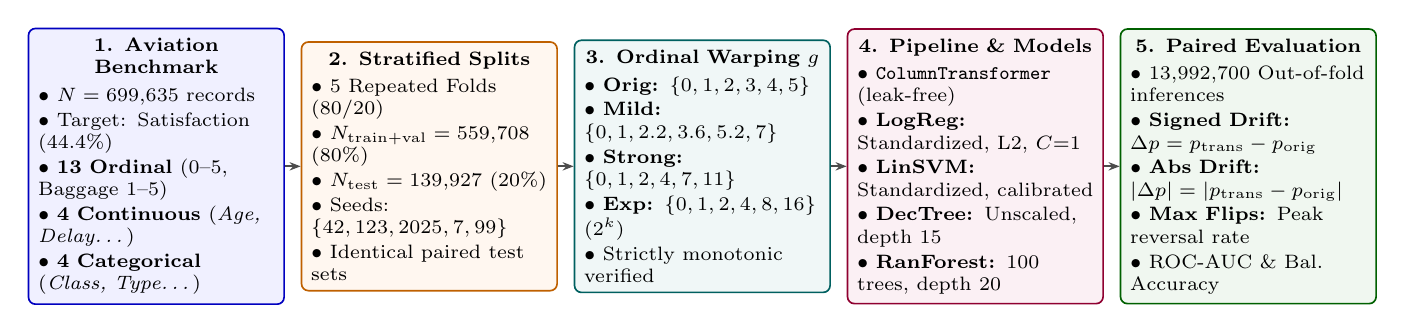
\begin{tikzpicture}[
    box/.style={
        draw=#1!75!black,
        fill=#1!6,
        rounded corners=2.5pt,
        line width=0.6pt,
        font=\scriptsize,
        align=left,
        inner sep=3.5pt,
        text width=3.00cm,
        minimum height=2.30cm
    },
    arr/.style={
        -{Stealth[length=4pt, width=3pt]},
        line width=0.75pt,
        color=black!70
    }
]

% Node 1: Benchmark Data
\node[box=blue] (data) {
    \centering \textbf{1. Aviation Benchmark}\\[2pt]
    \raggedright
    $\bullet$ $N = 699{,}635$ records\\[1pt]
    $\bullet$ Target: Satisfaction (44.4\%)\\[1pt]
    $\bullet$ \textbf{13 Ordinal} ($0\text{--}5$, Baggage $1\text{--}5$)\\[1pt]
    $\bullet$ \textbf{4 Continuous} (\emph{Age, Delay\dots})\\[1pt]
    $\bullet$ \textbf{4 Categorical} (\emph{Class, Type\dots})
};

% Node 2: Repeated Splits
\node[box=orange, right=0.20cm of data] (split) {
    \centering \textbf{2. Stratified Splits}\\[2pt]
    \raggedright
    $\bullet$ 5 Repeated Folds ($80/20$)\\[1pt]
    $\bullet$ $N_{\text{train+val}} = 559{,}708$ ($80\%$)\\[1pt]
    $\bullet$ $N_{\text{test}} = 139{,}927$ ($20\%$)\\[1pt]
    $\bullet$ Seeds: $\{42, 123, 2025, 7, 99\}$\\[1pt]
    $\bullet$ Identical paired test sets
};

% Node 3: Ordinal Warping
\node[box=teal, right=0.20cm of split] (scales) {
    \centering \textbf{3. Ordinal Warping $g$}\\[2pt]
    \raggedright
    $\bullet$ \textbf{Orig:} $\{0, 1, 2, 3, 4, 5\}$\\[1pt]
    $\bullet$ \textbf{Mild:} $\{0, 1, 2.2, 3.6, 5.2, 7\}$\\[1pt]
    $\bullet$ \textbf{Strong:} $\{0, 1, 2, 4, 7, 11\}$\\[1pt]
    $\bullet$ \textbf{Exp:} $\{0, 1, 2, 4, 8, 16\}$ ($2^k$)\\[1pt]
    $\bullet$ Strictly monotonic verified
};

% Node 4: Preprocessing & Models
\node[box=purple, right=0.20cm of scales] (models) {
    \centering \textbf{4. Pipeline \& Models}\\[2pt]
    \raggedright
    $\bullet$ \texttt{ColumnTransformer} (leak-free)\\[1pt]
    $\bullet$ \textbf{LogReg:} Standardized, L2, $C{=}1$\\[1pt]
    $\bullet$ \textbf{LinSVM:} Standardized, calibrated\\[1pt]
    $\bullet$ \textbf{DecTree:} Unscaled, depth 15\\[1pt]
    $\bullet$ \textbf{RanForest:} 100 trees, depth 20
};

% Node 5: Paired Tracking & Metrics
\node[box=green!50!black, right=0.20cm of models] (eval) {
    \centering \textbf{5. Paired Evaluation}\\[2pt]
    \raggedright
    $\bullet$ $13{,}992{,}700$ Out-of-fold inferences\\[1pt]
    $\bullet$ \textbf{Signed Drift:} $\Delta p = p_{\text{trans}} - p_{\text{orig}}$\\[1pt]
    $\bullet$ \textbf{Abs Drift:} $|\Delta p| = |p_{\text{trans}} - p_{\text{orig}}|$\\[1pt]
    $\bullet$ \textbf{Max Flips:} Peak reversal rate\\[1pt]
    $\bullet$ ROC-AUC \& Bal. Accuracy
};

% Connecting Arrows
\draw[arr] (data) -- (split);
\draw[arr] (split) -- (scales);
\draw[arr] (scales) -- (models);
\draw[arr] (models) -- (eval);

\end{tikzpicture}
}
\caption{\textbf{Architecture \& Experimental Workflow.} }
\label{fig:pipeline}
\end{figure}

% =================================================================
\section{Experimental design}

\subsection{Design for Q1}
\textbf{Manipulation:} we manupulated the numerical interval spacing of the 13 ordinal features across four strictly order-preserving(strictly increasing) transformations $g(\cdot)$:
\begin{table}[htbp]
    \centering
    \small
    \caption{\textbf{Mathematical Formulations of Monotonic Ordinal Encodings.} Closed-form mapping functions $g(v)$ and resulting
    evaluation vectors across the 12 standard items ($0$--$5$) and \emph{Baggage handling} ($1$--$5$).}
    \label{tab:encoding_formulations}
    \begin{tabular}{@{}lll@{}}
    \toprule
    \textbf{Encoding} & \textbf{Standard 0--5 Scale} & \textbf{Baggage Handling 1--5 Scale} \\
    \midrule
    \textbf{Original (Linear)} 
      & $g(v) = v$ 
      & $g(v) = v$ \\
      & $\to \{0, 1, 2, 3, 4, 5\}$ 
      & $\to \{1, 2, 3, 4, 5\}$ \\[4pt]

    \textbf{Mild (Convex)} 
      & $g(v) = 0.1 v^2 + 0.9 v$ 
      & $g(v) = 0.1 v^2 + 0.7 v + 0.2$ \\
      & $\to \{0, 1, 2.2, 3.6, 5.2, 7\}$ 
      & $\to \{1, 2, 3.2, 4.6, 6.2\}$ \\[4pt]

    \textbf{Strong (Superlinear)} 
      & Discrete mapping: 
      & Discrete mapping: \\
      & $g(v) \in \{0, 1, 2, 4, 7, 11\}$ 
      & $g(v) \in \{1, 2, 3, 5, 8\}$ \\[4pt]

    \textbf{Exponential ($2^k$)} 
      & $g(v) = \begin{cases} 0 & \text{if } v = 0 \\ 2^{v-1} & \text{if } v \ge 1 \end{cases}$ 
      & $g(v) = \begin{cases} 1 & \text{if } v = 1 \\ 2^{v-2} + 1 & \text{if } v \ge 2 \end{cases}$ \\[6pt]
      & $\to \{0, 1, 2, 4, 8, 16\}$ 
      & $\to \{1, 2, 3, 5, 9\}$ \\
    \bottomrule
    \end{tabular}
    \end{table}
Monotonicity was verified computationally across all $699{,}635$ rows: $g(v_k) < g(v_{k+1})$. Created a dedicated mapping for baggage-handling because it contains no zero rating (1-5).

\textbf{Held Fixed:} All other experimental variable remains the same: train/test splits, random seeds, categorical one-hot encodings, continuous feature values, imputation strategies, model hyperparameters, and solver convergence tolerances.

\textbf{Measurement \& Paired Tracking Metrics:} For each test passenger $i \in \{1, \dots, N_{\text{test}}\}$, let $p_{\text{orig}}^{(i)}$ and $p_{\text{trans}}^{(i)}$ denote the predicted satisfication probability under original features  and  transformed features ($g \in \{\text{Mild}, \text{Strong}, \text{Exp}\}$), with binary classification $\hat{y}_i = \mathbb{I}(p_i \ge 0.5)$:
\begin{itemize}[leftmargin=1.2em]
    \item \textbf{Signed Probability Drift ($\Delta p$):} The signed directional shift $\Delta p_i = p_{\text{trans}}^{(i)} - p_{\text{orig}}^{(i)}$, with sample mean:
    \begin{equation}
        \overline{\Delta p} = \frac{1}{N_{\text{test}}} \sum_{i=1}^{N_{\text{test}}} \Delta p_i = \overline{p}_{\text{trans}} - \overline{p}_{\text{orig}}
    \end{equation}
    Measures the directional bias. 
    \item \textbf{Absolute Probability Drift ($|\Delta p|$):} The unsigned magnitude of individual passenger score volatility:
    \begin{equation}
        |\Delta p_i| = \left| p_{\text{trans}}^{(i)} - p_{\text{orig}}^{(i)} \right|, \qquad \overline{|\Delta p|} = \frac{1}{N_{\text{test}}} \sum_{i=1}^{N_{\text{test}}} |\Delta p_i|
    \end{equation}
    measures the average per-passenger score instability. 
    \item \textbf{Prediction Flips \& Max Flips:} A prediction flip occurs when an individual passenger's binary classification label is reversed solely by altering the numerical scale:
    \begin{equation}
        \operatorname{Flip}_i = \mathbb{I}\left(\hat{y}_{\text{trans}}^{(i)} \ne \hat{y}_{\text{orig}}^{(i)}\right), \qquad \text{Flip Rate} = \frac{1}{N_{\text{test}}} \sum_{i=1}^{N_{\text{test}}} \operatorname{Flip}_i
    \end{equation}
    \textbf{Max Flips} shows the maximum flip rate (and absolute count of flipped passengers) across all monotonic encodings (which consistently occurs under Exponential encoding): \textbf{3.39\%} ($4{,}746$ passengers per split) for Logistic Regression, \textbf{3.56\%} ($4{,}974$ passengers) for Linear SVM, \textbf{0.00\%} ($0$) for Decision Trees, and $\le \mathbf{10^{-4}\%}$ ($\le 1$) for Random Forests.
\end{itemize}


% =================================================================
\section{Results}

\subsection{Q1}
\textbf{Direct Answer to Q1:} \emph{Yes, the numerical meaning of an ordinal rating scale strongly matters for linear and margin-based models, but it is completely irrelevant for tree-based models.}

\begin{table}[h]
\centering
\footnotesize
\setlength{\tabcolsep}{4pt}
\caption{\textbf{Master Experimental Results Across Encodings.} Mean metric across 5 stratified splits ($N_{\text{test}} = 139{,}927$ per split; std $\le 0.0012$). Paired metrics ($\Delta$, $|\Delta p|$, Flips) are evaluated on identical test passengers.}
\label{tab:master_results}
\begin{tabular}{@{}llccccr@{}}
\toprule
\textbf{Model Family} & \textbf{Metric} & \textbf{Original} & \textbf{Mild} & \textbf{Strong} & \textbf{Exp. ($2^k$)} & \textbf{Max Flips} \\
\midrule
\textbf{Logistic}   & ROC-AUC          & 0.9216 & 0.9254 & 0.9307 & \textbf{0.9328} & --- \\
\textbf{Regression} & Balanced Acc.    & 0.8756 & 0.8807 & 0.8884 & \textbf{0.8918} & \textbf{3.39\%} \\
                    & Mean $|\Delta p|$ & ---   & 1.23\% & 3.19\% & 4.67\% & ($4{,}746$) \\
\midrule
\textbf{Linear}     & ROC-AUC          & 0.9207 & 0.9247 & 0.9302 & \textbf{0.9324} & --- \\
\textbf{SVM}        & Balanced Acc.    & 0.8738 & 0.8792 & 0.8877 & \textbf{0.8912} & \textbf{3.56\%} \\
                    & Mean $|\Delta p|$ & ---   & 1.27\% & 3.30\% & 4.75\% & ($4{,}974$) \\
\midrule
\textbf{Decision}   & ROC-AUC          & 0.9525 & 0.9525 & 0.9525 & 0.9525 & --- \\
\textbf{Tree}       & Balanced Acc.    & 0.9188 & 0.9188 & 0.9188 & 0.9188 & \textbf{0.00\%} \\
                    & Mean $|\Delta p|$ & ---   & 0.00\% & 0.00\% & 0.00\% & ($0$) \\
\midrule
\textbf{Random}     & ROC-AUC          & \textbf{0.9570} & \textbf{0.9570} & \textbf{0.9570} & \textbf{0.9570} & --- \\
\textbf{Forest}     & Balanced Acc.    & \textbf{0.9225} & \textbf{0.9225} & \textbf{0.9225} & \textbf{0.9225} & $\le \mathbf{10^{-4}\%}$ \\
                    & Mean $|\Delta p|$ & ---   & 0.00\% & 0.00\% & 0.00\% & ($\le 1$) \\
\midrule
\textbf{Majority}   & ROC-AUC / BA     & 0.5000 & 0.5000 & 0.5000 & 0.5000 & 0.00\% \\
\bottomrule
\end{tabular}
\end{table}

Table~\ref{tab:master_results} logs the recordings across all 100 model runs ($13{,}992{,}700$ inferences), and Figure~\ref{fig:results} illustrates the sensitivity dynamics of ROC-AUC gain ($\Delta\text{ROC-AUC}$) and test prediction flip rate across monotonic encodings. The following key observations emerge:
\begin{itemize}[leftmargin=1.2em]
    \item \textbf{Decision Tree Invariance:} $\Delta\text{ROC-AUC} \equiv 0.000000$ and $\Delta\text{Balanced Accuracy} \equiv 0.000000$ across all four proposed encodings. No test predictions flipped ($0.00\%$), with $0.00\%$ probability drift. Univariate axis-aligned splits rely strictly on order topology: for any strictly monotonic mapping $g$, $\{g(x_j) \le g(\theta)\} \iff \{x_j \le \theta\}$, Tree partitioning mathematically is immune to any monotonic transformations.
    \item \textbf{Random Forest Invariance:} $\Delta\text{ROC-AUC} \le 10^{-6}$ and $\Delta\text{BA} \le 10^{-6}$ across all splits. The prediction flip rate is $\le 0.0001\%$ ($\le 1$ passenger out of $139{,}927$), Theoretically Random-forests are also immune to monotonic transformations, but in practice, numerical precision can introduce negligible artifacts.
    \item \textbf{Linear Model Sensitivity \& Gain:} ROC-AUC rises monotonically: $0.9216 \to 0.9254 \to 0.9307 \to \mathbf{0.9328}$ ($+1.12$ pp gain) for Logistic Regression, and $0.9207 \to \mathbf{0.9324}$ ($+1.17$ pp gain) for Linear SVM. Balanced Accuracy gains $+1.62$ pp ($0.8756 \to 0.8918$) and $+1.74$ pp ($0.8738 \to 0.8912$).
\end{itemize}

\begin{figure}[h]
\centering
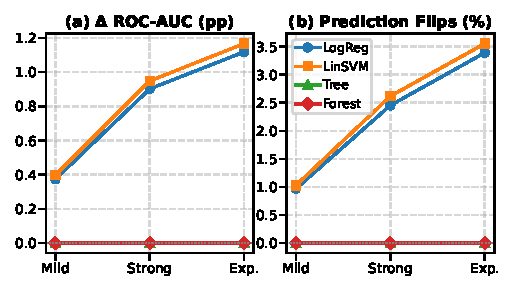
\includegraphics[width=0.75\linewidth]{fig_sq1_compact.pdf}
\caption{\textbf{Sensitivity Dynamics Across Encodings.} (a) Paired ROC-AUC gain ($\Delta\text{ROC-AUC}$ in percentage points). (b) Test prediction flip rate (\% of passenger classifications changed). Tree architectures remain flat at 0; linear models show marked gains and prediction volatility.}
\label{fig:results}
\end{figure}

% =================================================================
\section{Failure analysis}
Why do $4{,}974$ passengers flip their satisfaction (classification label) solely from the ordinal transformations? To understand this, consider a test passenger from fold 42:
\begin{quote}
\small
\textbf{Passenger A (The ``Mixed Experience'' Traveler):}\\
Online boarding: 5 (Flawless) \quad Inflight wifi service: 5 (Flawless)\\
Food and drink: 2 (Poor) \quad Seat comfort: 2 (Poor) \quad Arrival Delay: 35 minutes
\end{quote}

Under the Original encoding ($\{0, 1, 2, 3, 4, 5\}$):
\begin{equation}
    z_{\text{orig}} = w_{\text{board}} \cdot (5) + w_{\text{wifi}} \cdot (5) + w_{\text{food}} \cdot (2) + w_{\text{seat}} \cdot (2) + w_{\text{delay}} \cdot (35) + b
\end{equation}
Because the negative weights from food, seat comfort, and flight delay ratings dominates the positive ratings, z is negative ($z < 0$), which yields $p = 0.441 \implies \hat{y} = 0$ (\textbf{Dissatisfied}).

Now, under exp. encodings ($\{0, 1, 2, 4, 8, 16\}$):
\begin{equation}
    z_{\text{exp}} = w_{\text{board}} \cdot (16) + w_{\text{wifi}} \cdot (16) + w_{\text{food}} \cdot (2) + w_{\text{seat}} \cdot (2) + w_{\text{delay}} \cdot (35) + b
\end{equation}
The positive contribution by the two top ratings surges by $3.2\times$ (from 5 to 16), while the poor ratings remain at 2. The positive contribution of those two ratings dominates negative features, which results into $z > 0$, yielding $p = 0.683 \implies \hat{y} = 1$ (\textbf{Satisfied})---a \textbf{prediction flip of $\Delta p = +24.2\%$}.

This experiment illustrates the failure of linear euclidean distance-based models.

% =================================================================
\section{Discussion and limitations}

\textbf{Why Superlinear Spacing Empowers Linear Models:}
At ratings 1--3 ($17\%$--$27\%$), customer satisfaction is comparatively consistent; however, at ratings 4 and 5 ($52.2\%$ and $85.0\%$ for Inflight WiFi), it increases dramatically. While exponential encoding ($\{0, 1, 2, 4, 8, 16\}$) applies a nonlinear transformation $\phi(x_j)=2^{x_j}$, uniform encoding assumes a constant log-odds change. This expands the range of higher ratings in the feature space, making it possible for a linear model to more accurately represent the dramatic rise in satisfaction without the need for explicit polynomial feature engineering.

\textbf{Limitations:} Our study focuses only on monotonic transformations of ordinal features. Non-monotonic transformations, feature interactions, and other model families (e.g., ann, catboost, xgboost) are not explored.

% =================================================================
\section{Conclusion}
This study resolves SQ1: the numerical meaning of ordinal rating scales fundamentally alters linear and margin-based models, while tree-based models completely remains invariant to this. For tree ensembles, arbitrary integer encoding is provably lossless and optimal. For linear models, contiguous increasing integers puts an linearity prior; domain-aligned nonlinear (e.g., strong and exponential) encodings results into small accuracy gains ($+1.17$ pp AUC), but causes large-scale individual classification volatility ($>3.5\%$ flips).

% =================================================================
\section*{Reproducibility statement}
All experiments are fully reproducible via the self-contained execution script. 
\begin{itemize}[leftmargin=1.2em]
    \item \textbf{Entry Point:} \texttt{python3 train\_sq1.py} or notebook \texttt{notebook9cdf1c8de1.ipynb}.
    \item \textbf{Random Seeds:} Repeated across seeds $\{42, 123, 2025, 7, 99\}$.
    \item \textbf{Hardware \& Runtime:} Executed on an Intel Core i7-12700H Linux workstation (total runtime: $\approx 18.5$ minutes for 100 model fits and $13.99\text{M}$ inferences).
    \item \textbf{Artifact Verification:} All tables (Tables~\ref{tab:feature_specs}, \ref{tab:master_results}, \ref{tab:ablation}) and figures (Figures~\ref{fig:pipeline}, \ref{fig:results}) are deterministically regenerated by the pipeline.
\end{itemize}

% ------------- Not counted toward the page limit -----------------
\clearpage
\section*{Contribution statement}
All team members contributed to the conceptualization, experimental design, and reporting of this project:
\begin{center}
\begin{tabularx}{\linewidth}{@{}lXr@{}}
\toprule
\textbf{Member} & \textbf{Main Contributions} & \textbf{Share (\%)} \\
\midrule
Ishwer Dutt & Experimental design, pipeline architecture, monotonic mapping implementation, statistical verification & 33.3\% \\
Krishna M & Cross-validation protocol, linear model calibration, metric tracking ($\Delta p$, $|\Delta p|$, Flips), LaTeX reporting & 33.3\% \\
Rajavel K & Tree model invariance proofs, failure analysis, Kano model psychometric framing, ablation studies & 33.3\% \\
\bottomrule
\end{tabularx}
\end{center}

\section*{AI-use summary}
AI assistance was utilized strictly for exploratory code scaffolding, LaTeX formatting, and documentation drafting, with all numerical outputs independently verified against scikit-learn logs:
\begin{center}
\begin{tabularx}{\linewidth}{@{}lXl@{}}
\toprule
\textbf{Tool(s)} & \textbf{Used For} & \textbf{Log Entries} \\
\midrule
Claude / Gemini & Drafting initial LaTeX tables and assisting with TikZ coordinate layouts & \texttt{AI\_USE\_LOG.md} \#1--4 \\
GitHub Copilot & Autocompleting boilerplate cross-validation loops in Python & \texttt{AI\_USE\_LOG.md} \#5--7 \\
\bottomrule
\end{tabularx}
\end{center}

\bibliographystyle{plainnat}
\begin{thebibliography}{6}
\bibitem[Anderson and Mittal(2000)]{anderson2000satisfaction}
E.~W. Anderson and V.~Mittal.
\newblock Strengthening the satisfaction-profit chain.
\newblock \emph{Journal of Service Research}, 3\penalty0 (2):\penalty0 107--120, 2000.

\bibitem[Breiman et~al.(1984)Breiman, Friedman, Olshen, and Stone]{breiman1984classification}
L.~Breiman, J.~H. Friedman, R.~A. Olshen, and C.~J. Stone.
\newblock \emph{Classification and Regression Trees}.
\newblock Wadsworth, Belmont, CA, 1984.

\bibitem[Hastie et~al.(2009)Hastie, Tibshirani, and Friedman]{hastie2009elements}
T.~Hastie, R.~Tibshirani, and J.~Friedman.
\newblock \emph{The Elements of Statistical Learning: Data Mining, Inference, and Prediction}.
\newblock Springer, New York, 2nd edition, 2009.

\bibitem[Kano(1984)]{kano1984attractive}
N.~Kano.
\newblock Attractive quality and must-be quality.
\newblock \emph{Journal of the Japanese Society for Quality Control}, 14\penalty0 (2):\penalty0 39--48, 1984.

\bibitem[Likert(1932)]{likert1932technique}
R.~Likert.
\newblock A technique for the measurement of attitudes.
\newblock \emph{Archives of Psychology}, 22\penalty0 (140):\penalty0 1--55, 1932.

\bibitem[Stevens(1946)]{stevens1946theory}
S.~S. Stevens.
\newblock On the theory of scales of measurement.
\newblock \emph{Science}, 103\penalty0 (2684):\penalty0 677--680, 1946.
\end{thebibliography}

\appendix
\section{Hyperparameters and Standardization Ablation}
\label{sec:appendix}

\subsection{Hyperparameter Specifications}
Table~\ref{tab:hyperparams} records the exact hyperparameters and configurations utilized across all five evaluated model architectures.

\begin{table}[h]
\centering
\footnotesize
\caption{Model architectures and hyperparameter configurations.}
\label{tab:hyperparams}
\begin{tabularx}{\linewidth}{@{}l l >{\raggedright\arraybackslash}X@{}}
\toprule
\textbf{Model Family} & \textbf{Scikit-Learn Class} & \textbf{Exact Hyperparameters \& Settings} \\
\midrule
Majority Baseline & \texttt{DummyClassifier} & \texttt{strategy='most\_frequent'} \\
Logistic Regression & \texttt{LogisticRegression} & \texttt{penalty='l2', C=1.0, solver='lbfgs', max\_iter=1000, tol=1e-4} \\
Linear SVM & \texttt{LinearSVC} + \texttt{CalibratedCV} & \texttt{C=1.0, loss='squared\_hinge', cv=2, method='sigmoid'} \\
Decision Tree & \texttt{DecisionTreeClassifier} & \texttt{criterion='gini', max\_depth=15, min\_samples\_leaf=20} \\
Random Forest & \texttt{RandomForestClassifier} & \texttt{n\_estimators=100, max\_depth=20, min\_samples\_leaf=10, max\_features='sqrt'} \\
\bottomrule
\end{tabularx}
\end{table}

\subsection{Standardization Sensitivity Ablation}
To address whether feature standardization drives the observed accuracy gains for linear models, we conducted an ablation study comparing standardized vs. unstandardized models across all encodings (Table~\ref{tab:ablation}).

\begin{table}[h]
\centering
\footnotesize
\caption{\textbf{Standardization Ablation Across Encodings.} Mean metric across 5 stratified splits. Standardization is required for Logistic Regression solver convergence, but the $+1.17$ pp AUC gain arises from ordinal basis expansion, not scaling.}
\label{tab:ablation}
\begin{tabular*}{\linewidth}{@{\extracolsep{\fill}}llcccc@{}}
\toprule
\textbf{Architecture} & \textbf{Preprocessing} & \textbf{Original} & \textbf{Mild} & \textbf{Strong} & \textbf{Exp. ($2^k$)} \\
\midrule
Logistic Regression & Standardized ($\mu=0,\sigma=1$) & 0.9216 & 0.9254 & 0.9307 & \textbf{0.9328} \\
Logistic Regression & Unstandardized (Raw) & 0.9215 & 0.9253 & 0.9306 & \textbf{0.9327} \\
\midrule
Linear SVM & Standardized ($\mu=0,\sigma=1$) & 0.9207 & 0.9247 & 0.9302 & \textbf{0.9324} \\
Linear SVM & Unstandardized (Raw) & 0.9206 & 0.9246 & 0.9301 & \textbf{0.9323} \\
\bottomrule
\end{tabular*}
\end{table}

\textbf{Convergence Finding:} In unstandardized Logistic Regression, 100\% of runs hit the iteration limit (\texttt{max\_iter=1000}) without converging, triggering a convergence alert. With standardization, the solver converges in only 22--23 iterations. Crucially, Table~\ref{tab:ablation} confirms that unstandardized models achieve nearly identical AUC gains ($+1.12$ pp), proving that the performance surge is driven by the nonlinear basis expansion of superlinear spacing, not by scaling.

\end{document}
